

\noindent
\label{sec:dfp}
IBM’s Data Fabrication Platform (DFP) is a web based central platform that provides a consistent and organisational-wide methodology (\emph{rule-guided fabrication}) for generating high-quality data for testing, development, and training. Fabrication of synthetic data consists of two stages - \emph{data modelling} and \emph{data generation}. Furthermore, data modelling comprises \emph{resources and structure definitions}, \emph{constraint rules definitions} and \emph{fabrication configuration definitions}. Input and output resources are standard relational databases (e.g., DB2, Oracle, PostgreSQL, SQLite), standard file formats (e.g., Flat file, XLS, CSV, XML, JSON) and streaming via MQTT protocol.

In rule guided fabrication, the database logic is extracted automatically and is augmented by application logic and testing logic modelled by the user. The application logic and the testing logic can be modelled using rules that the platform provides, but the users can also add new rules. Once the user requests the generation of a certain amount of data into a set of test databases, the platform internally ensures that the generated data satisfies the modelled rules as well as the internal databases consistency requirements. The platform can generate data from scratch, inflate existing databases, move existing data, and transform data from previously existing resources, such as old test databases or even production data. The platform provides a comprehensive and hybrid solution that can create a mixture of synthetic and real data according to user requirements.

\begin{figure}
    \centering
    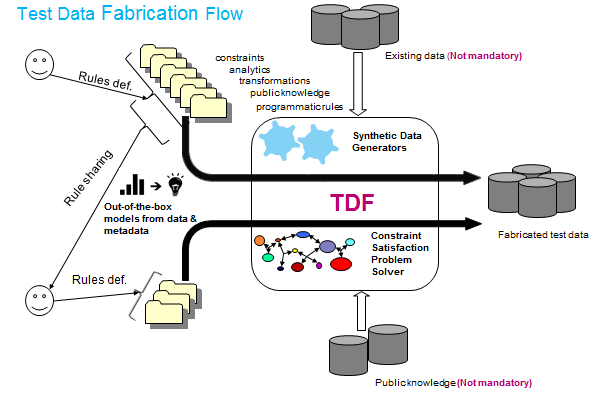
\includegraphics[width=0.45\textwidth]{images/DFPPlatformFlow.png}
    \caption{Flow of Generating Fabricated Data}
    \label{fig:dataFab}
\end{figure}

To overcome the shortcomings of existing data generation techniques, DFP generates data using a proprietary \emph{Constraint Satisfaction Problem (CPS)} solver (See Figure~\ref{fig:dataFab}). This methodology is generic and does not require access to real data, making it very safe to use in our setting. Data fabrication consists of the following steps.
\begin{enumerate}
\item The user defines a data project which contains the structure of the data, the constraint rules and the fabrication configuration. In order to construct a constraint satisfaction problem for the solver, the platform analyses the table metadata to get the desired properties (columns data types, referential integrity constraints etc.). 
\item The platform then selects a subset of the relevant rules and tables using the fabrication configuration, with possible addition of relevant parent tables and some default rules (e.g. PK and Unique Column). This information is used for the construction of a database table dependency graph. For each table in that graph, starting at root nodes, structural record dependencies are built recursively.
\item Based on the dependency graph, the fabrication pattern is computed where each target table record is assigned to one of the following fabrication modes: ‘New’, ‘Reuse’ or ‘Other’. Given the patterns, the graph and the rules, a CSP problem can be created. The problem consists of variables and rules, and a solution is an assignment of values to variables that satisfies the rules. 
\item Finally, the CSP problem is submitted to the solver, which produces a desired number of solutions to the problem and stores them in the appropriate places (e.g.~database, file or stream).
\end{enumerate} 

